\section{Emanuel Sujeta}

\subsection{Sample photo and text}

\begin{figure}[htpb] %dzieki temu obrazek pojawia się tam gdzie chcemy, a nie na samej górze ;))
    \centering
    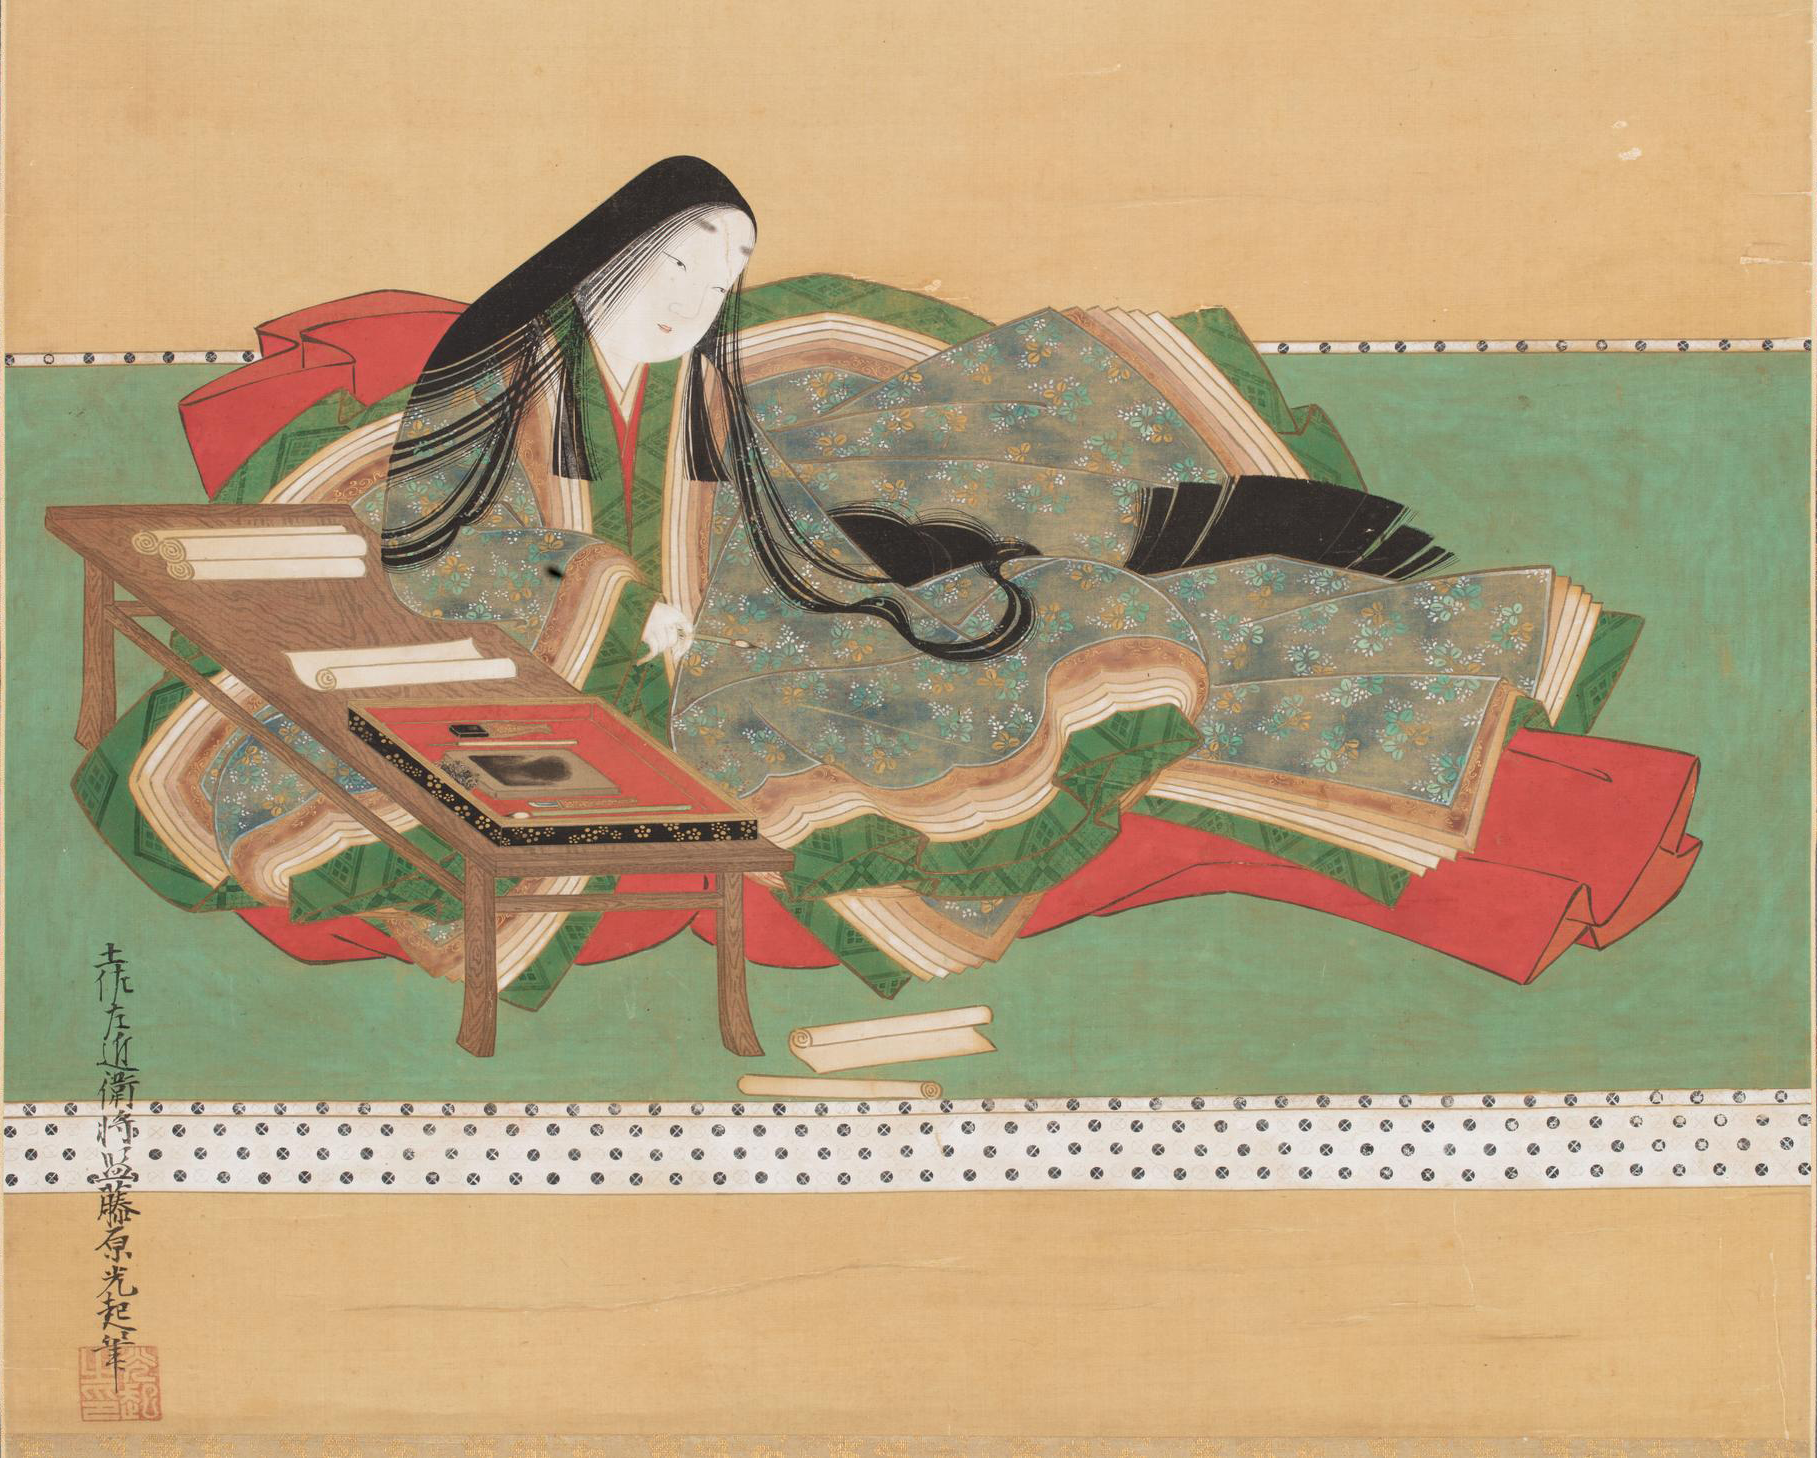
\includegraphics[width=1\textwidth]{pictures/Murasaki-Shikibu.png}
    \caption{\textbf{Murasaki Shikibu} composing \emph{The Tale of Genji}}
    \label{fig:murasaki}
\end{figure}

\textbf{Murasaki Shikibu} (Rysunek~\ref{fig:murasaki}) was a Japanese novelist, poet and lady-in-waiting at the Imperial court in the Heian period. She is best known as the author of \emph{The Tale of Genji}, widely considered to be one of the world's first novels, written in Japanese between about 1000 and 1012.

\subsection{Sample table}

\begin{table}[htpb]
    \centering
    \caption{2022 \underline{Fijian} general election results:}
    \begin{tabular}{|c|c|c|c|c|c|} \hline 
         Party& Votes& \%& +/-& Seats& +/-\\ \hline
         FijiFirst& 200,246& 42.55& -7.47& 26& -1\\ \hline
         People's Alliance& 168,581& 35.82& +35.82& 21& +21\\ \hline
         National Federation Party& 41,830& 8.89& +1.51& 5& +2\\ \hline
         Social Democratic Liberal Party& 24,172& 5.14& -34.71& 3& -18\\ \hline
         Unity Fiji Party& 13,100& 2.78& +1.26& 0& 0\\ \hline
         Fiji Labour Party& 12,704& 2.70& +2.08& 0& 0\\ \hline
         We Unite Fiji Party& 6,070& 1.29& +1,29& 0& 0\\ \hline
    \end{tabular}
    \label{tab:Fiji}
\end{table}

\subsection{Sample text}

\centerline{Lord's Prayer in Latin:}

\emph{\textbf{Pater noster}, qui es in caelis: sanctificétur nomen tuum; advéniat regnum tuum; fiat volúntas tua, sicut in caelo, et in terra. Panem nostrum cotidiánum da nobis hodie; et dimítte nobis débita nostra, sicut et nos dimíttimus debitóribus nostris; et ne nos indúcas in tentatiónem; sed líbera nos a malo. Amen.}

\subsection{Sample list}

\textbf{Best NBA players of all time:}

\begin{enumerate}
    \item Lebron James
    \item Michael Jordan
    \item Larry Bird
    \item Magic Johnson
    \item Bill Russel
    \item Kevin Durant
\end{enumerate}

\begin{itemize}
    \item Jeremiasz Sochan
\end{itemize}

\subsection{Sample math expression}

Wave equation in one space dimension:

\[\frac{\partial^2 u}{\partial t^2} = c^2 \frac{\partial^2 u}{\partial x^2}\]

